%%%%%%%%%%%%%%%%%%%%%%%%%%%%%%%%%%%%%%%%%%%%%%%%%%%%%%%%%%%%%%%%%%%%%%%%%%
% This is just an example/guide for you to refer to when submitting manuscripts to Frontiers, it is not mandatory to use Frontiers .cls files nor frontiers.tex
% This will only generate the Manuscript, the final article will be typeset by Frontiers after acceptance.
%
% When submitting your files, remember to upload this *tex file, the pdf generated with it, the *bib file (if bibliography is not within the *tex) and all the figures.
%%%%%%%%%%%%%%%%%%%%%%%%%%%%%%%%%%%%%%%%%%%%%%%%%%%%%%%%%%%%%%%%%%%%%%%%%%

%%% Version 3.4 Generated 2018/06/15 %%%
%%% You will need to have the following packages installed: datetime, fmtcount, etoolbox, fcprefix, which are normally inlcuded in WinEdt. %%%
%%% In http://www.ctan.org/ you can find the packages and how to install them, if necessary. %%%
%%%  NB logo1.jpg is required in the path in order to correctly compile front page header %%%

\documentclass[utf8]{frontiersSCNS} % for Science, Engineering and Humanities and Social Sciences articles
%\documentclass[utf8]{frontiersHLTH} % for Health articles
%\documentclass[utf8]{frontiersFPHY} % for Physics and Applied Mathematics and Statistics articles

%\setcitestyle{square} % for Physics and Applied Mathematics and Statistics articles
\usepackage{url,hyperref,lineno,microtype,subcaption}
\usepackage[onehalfspacing]{setspace}
\usepackage{siunitx}			% allows to use units in text

\linenumbers

% Leave a blank line between paragraphs instead of using \\

%%% no italics (in equations) using T{}
\newcommand{\T}[1]{\text{#1}}

%%%%%%%%%%%%%%%%%%%%%%%%%%%%%%%%%%%%%%%%%%%%%%%%%%%%%%%%%%%%%%%%%%%%%%%%%%
% Authorship
%%%%%%%%%%%%%%%%%%%%%%%%%%%%%%%%%%%%%%%%%%%%%%%%%%%%%%%%%%%%%%%%%%%%%%%%%%
\def\keyFont{\fontsize{8}{11}\helveticabold }
\def\firstAuthorLast{Richard Bachmaier {et~al.}} %use et al only if is more than 1 author
\def\Authors{Richard Bachmaier\,$^{1}$, Jörg Encke\,$^{1,2,3}$, Miguel Obando-Leitón\,$^{1,2,4}$, Werner Hemmert\,$^{1,2,4}$ and Siwei Bai\,$^{1,2,5,*}$}
% Affiliations should be keyed to the author's name with superscript numbers and be listed as follows: Laboratory, Institute, Department, Organization, City, State abbreviation (USA, Canada, Australia), and Country (without detailed address information such as city zip codes or street names).
% If one of the authors has a change of address, list the new address below the correspondence details using a superscript symbol and use the same symbol to indicate the author in the author list.
\def\Address{$^{1}$Department of Electrical and Computer Engineering, Technical University of Munich, 80333 Munich, Germany \\
$^{2}$Munich School of Bioengineering, Technical University of Munich, 85748 Garching, Germany \\
$^{3}$Medizinische Physik and Cluster of Excellence Hearing4all, Universität Oldenburg, 26111, Oldenburg, Germany\\
$^{4}$Graduate School of Systemic Neurosciences, Ludwig Maximilian University of Munich, 82152 Planegg, Germany \\
$^{5}$Graduate School of Biomedical Engineering, University of New South Wales, Sydney, NSW 2052, Australia  }
% The Corresponding Author should be marked with an asterisk
% Provide the exact contact address (this time including street name and city zip code) and email of the corresponding author
\def\corrAuthor{Siwei Bai}
\def\corrEmail{siwei.bai(at)tum.de}

%%%%%%%%%%%%%%%%%%%%%%%%%%%%%%%%%%%%%%%%%%%%%%%%%%%%%%%%%%%%%%%%%%%%%%%%%%
% Begin document
%%%%%%%%%%%%%%%%%%%%%%%%%%%%%%%%%%%%%%%%%%%%%%%%%%%%%%%%%%%%%%%%%%%%%%%%%%
\begin{document}
\onecolumn
\firstpage{1}

\title[Human ANF cable model comparison]{Comparison of multi-compartment cable models of human auditory nerve fibers}

\author[\firstAuthorLast ]{\Authors} %This field will be automatically populated
\address{} %This field will be automatically populated
\correspondance{} %This field will be automatically populated

\extraAuth{}% If there are more than 1 corresponding author, comment this line and uncomment the next one.
%\extraAuth{corresponding Author2 \\ Laboratory X2, Institute X2, Department X2, Organization X2, Street X2, City X2 , State XX2 (only USA, Canada and Australia), Zip Code2, X2 Country X2, email2@uni2.edu}

\maketitle

%%%%%%%%%%%%%%%%%%%%%%%%%%%%%%%%%%%%%%%%%%%%%%%%%%%%%%%%%%%%%%%%%%%%%%%%%%
% Abstract
%%%%%%%%%%%%%%%%%%%%%%%%%%%%%%%%%%%%%%%%%%%%%%%%%%%%%%%%%%%%%%%%%%%%%%%%%%
\begin{abstract}

\section{}
Background: Multi-compartment cable models of auditory nerve fibers have been developed to assist the improvement of cochlear implants. With the advancement of computational technology and the results obtained from in vivo and in vitro experiments, these models have evolved to incorporate a considerable degree of morphological and physiological details. They have also been combined with three-dimensional volume conduction models of the cochlea to simulate neural responses to electrical stimulation. However, no specific rules have been provided on choosing the appropriate cable model, and most models adopted in recent studies were chosen without a specific reason or by inheritance.

Methods: Three of the most cited biophysical multi-compartment cable models of the human auditory nerve, i.e. Rattay et al., Briaire and Friijns, and Smit et al., were implemented in this study. Several properties of single fibers were compared among the three models, including threshold, conduction velocity, action potential shape, latency, refractory properties, as well as stochastic and temporal behaviors. Experimental results regarding these properties were also included as a reference for comparison.

Results: For monophasic single-pulse stimulation, the ratio of anodic versus cathodic thresholds in all models was within the experimental range, despite a much larger ratio in the model by Briaire and Friijns. For biphasic pulse-train stimulation, thresholds as a function of both pulse rate and pulse duration differed between the models, but none matched the experimental observations even coarsely. Similarly, for all other properties including the conduction velocity, action potential shape, and latency, the models presented different outcomes and not all of them fell within the range observed in experiments.

Conclusions: While all three models presented similar values in certain single fiber properties to those obtained in experiments, none matched the experimental observations satisfactorily. In particular, the adaptation and temporal integration behaviors were completely missing in all models. Further extensions and analyses are required to explain and simulate realistic auditory nerve fiber responses to electrical stimulation.

\tiny
 \keyFont{ \section{Keywords:} Auditory nerve, computational model, biophysical, cable model, electrical stimulation, threshold} %All article types: you may provide up to 8 keywords; at least 5 are mandatory.
\end{abstract}

%%%%%%%%%%%%%%%%%%%%%%%%%%%%%%%%%%%%%%%%%%%%%%%%%%%%%%%%%%%%%%%%%%%%%%%%%%
% Introduction
%%%%%%%%%%%%%%%%%%%%%%%%%%%%%%%%%%%%%%%%%%%%%%%%%%%%%%%%%%%%%%%%%%%%%%%%%%
\section{Introduction}
\label{sec:introduction}
Multi-compartment cable models of the auditory nerve fibers (ANF) have been developed to assist in understanding and predicting neural responses to external stimulation. They have been used to advance our knowledge regarding how the auditory nerve encodes timing, frequency and intensity information \citep{Imennov2009}. Moreover, multi-compartment ANF models have %frequently 
been combined with three-dimensional volume conduction models of the cochlea to simulate responses to cochlear implant (CI) stimulation \citep{Kalkman2015,Malherbe2016,Nogueira2018}. Alongside psychophysical experiments, computational models of the auditory nerve are used to evaluate new sound coding and stimulation strategies and are therefore crucial for the improvement of CIs. Nevertheless, there exist several ANF models in the literature with varying  morphological or ionic channel properties. Choosing the appropriate cable model for a given computational study is difficult as the different models are difficult to compare based on the original publications. Consequently, most models adopted in existing studies were chosen without a specific reason or by inheritance.

Generally speaking, multi-compartment models are morphological extensions of single-node models. Based on the Schwarz–Eikhof (SE) node model of rat and feline ion channel kinetics \citep{Schwarz1987}, \cite{Frijns1994} developed an axon model, which was subsequently extended with dendrite and soma to match the feline ANF morphology \citep{Frijns1995}. However, differences in morphology between human and cat might impact spike travel time, and this must be taken into account for correct predictions of CI stimulus coding in humans \citep{Rattay2001,OBrien2016}. Therefore, this feline ANF model was later modified to account for the human ANF morphology \citep{Briaire2005}. Meanwhile, \cite{Rattay2001} designed a different human ANF model based on Hodgkins and Huxleys (HH) description of the unmyelinated squid axon \citep{Hodgkin1952} while also including human ANF morphology. \cite{Smit2008} adopted the dendrite and soma from \cite{Rattay2001}, but modified the properties of the axon in order to account for differences in membrane currents at the node of Ranvier between human \citep{Schwarz1995} and squid.

In addition to differences in morphology and ion channel properties, some ANF cable models also include modifications in order to implement specific physiological properties, including stochastic effects and adaptation. For instance, \cite{Rattay2001} incorporated a simple and efficient approach to predict stochastic ANF responses by adding a Gaussian noise current term to the total ion current. In comparison, \cite{Imennov2009} and \cite{Negm2014} represented the stochastic nature of ion channels by applying a channel-number tracking algorithm. \cite{Woo2010} included a model of rate adaptation based on a dynamic external potassium concentration, whereas \cite{VanGendt2016} integrated their biophysical model with a phenomenological approach to simulate threshold fluctuations, adaptation and accommodation.

Differences in the description of ANF morphology and physiology lead to distinct model characteristics. A meaningful comparison based on the respective publications is however not feasible, as the models were only fitted to specific ANF properties under certain stimulation patterns. For example, \cite{Rattay2001} detailed the initiation and propagation of action potentials (APs), but did not describe properties like the strength-duration relation and refractory period. \cite{Frijns1994} and \cite{Smit2008} measured the AP shape, conduction velocity, strength-duration relation and refractory period, but none of these properties was mentioned for the updated versions of their model in \cite{Briaire2005} and \cite{Smit2010}. Studies that included an adaptation mechanism in their ANF cable models, investigated almost exclusively responses to pulse-train stimulation, but did not include single-pulse responses as in other studies. Therefore, it is necessary to compare the spiking characteristics of different ANF models in order to investigate how the models behave with more generalised stimuli. In this study, the three often cited biophysical human ANF cable models. The Rattay (RA) model from \cite{Rattay2001}, the Briaire-Frijns (BF) model from \cite{Briaire2005} and the Smit-Hanekom (SH) model from \cite{Smit2010}, were chosen and implemented in a consistent framework, and their performance was evaluated by comparing them against experimental data.

%%%%%%%%%%%%%%%%%%%%%%%%%%%%%%%%%%%%%%%%%%%%%%%%%%%%%%%%%%%%%%%%%%%%%%%%%%
% Methods
%%%%%%%%%%%%%%%%%%%%%%%%%%%%%%%%%%%%%%%%%%%%%%%%%%%%%%%%%%%%%%%%%%%%%%%%%%
\section{Methods}
\label{sec:methods}
The multi-compartment ANF models by \cite{Rattay2001}, \cite{Briaire2005} and \cite{Smit2010}, from here on abbreviated as RA, BF and SH, respectively, were implemented in a single framework using Python 3.4, with the package Brian2 \citep{Goodman2009}. All models followed the morphology of a human ANF as described in the original publication and consisted of dendrite, soma, and axon. Dendrite and axon were composed of an alternating structure of active nodes and passive myelinated internodes. Additionally, all models included a peripheral terminal as well as a pre-somatic region. All morphological components were modelled as electrical circuits and represented by cylindrical compartments. The spherical shape of the somas in the RA and SH models was approximated by segmenting it into ten cylindrical compartments. Compartment lengths and diameters were distinct in each model, as shown in Fig \ref{fig:morphologies}. Details of the morphologies can be taken from their respective publications. The length of dendritic internodes in \cite{Briaire2005} was defined as scalable so as to reflect the varied lengths from the organ of Corti to the soma. In this study, the dendritic internodes were scaled as suggested by \cite{Kalkman2014a} with a maximum length of \SI{250}{\micro\meter}.

In unmyelinated compartments of the ANF models, the cell membrane was represented by a capacitor which was charged or discharged by ionic currents. These currents depended on membrane's ionic permeabilities and Nernst potentials of individual ion species. All three models included exclusively sodium and potassium channels. The BF model utilised the gating properties suggested by \cite{Schwarz1987} and calculated the ionic currents according to \cite{Frankenhaeuser1964}, whereas RA and SH adopted the gating properties and equations proposed by \cite{Hodgkin1952}. However, compared to the original gating properties of the Hodgkin-Huxley (HH) kinetics, which were measured in a squid at \SI{6.3}{\celsius}, in the RA and SH models they were each multiplied by a compensating factor to account for the faster gating processes in mammalian nerve fibers, and the ionic channel densities were increased. Furthermore, in order to specifically account for the human ANF physiology, \cite{Smit2010} added two modifications to the HH ion channels in the axon: \emph{a)} the opening and closing of the potassium channels were modified to be slower \citep{Smit2008}; \emph{b)} a persistent sodium current was added to account for the total sodium current together with a transient one of the original HH model \citep{Smit2009}. While the models by \cite{Briaire2005} and \cite{Smit2010} are deterministic, \cite{Rattay2001} incorporated a simple approach to predict stochastic ANF responses by adding a Gaussian noise current term to the total ion current. It was calculated with:
\begin{equation}
i_{noise} = X \cdot k_{\T{noise}} \sqrt{A g_{\T{Na}}},
\label{equ:stochasticity_rattay}
\end{equation}
where $X$ is a Gaussian random variable (mean=0, S.D.=1). $g_{\T{Na}}$ denotes the maximum sodium conductivity, and $A$ is the membrane surface area. The term is multiplied with the factor $k_{\T{noise}}$, which is common to all compartments and is used to adjust how strongly the stochastic behavior of the channels is emphasized. In this study, we decided to add the noise term to all three models to investigate the feasibility of this approach to simulate stochasticity and to compare the models also with stochasticity.

Regarding the passive internodes, \cite{Briaire2005} implied that they were surrounded by a perfectly insulating myelin sheath. As a consequence, both their capacity and conductivity were assumed to be zero; whereas \cite{Rattay2001} described them as a passive resistor-capacitor network and thus as imperfect insulators. In \cite{Smit2010}, the dendritic internodes were modeled following \cite{Rattay2001}, but the axonal internodes were described using a double-cable structure as proposed by \cite{Blight1985}. Detailed information regarding the ionic models can again be found in the respective publications.

The extracellular space of the ANF models was simulated as a homogeneous medium with an isotropic resistivity of \SI{3}{\ohm\meter}. Unless otherwise stated, each fiber was stimulated externally by a point electrode situated above the third dendritic node with a vertical distance of \SI{500}{\micro\meter} to the fiber. Measurements were performed at the tenth axonal node to ensure the propagation of an action potential (AP) to the axon. Several properties of single ANF were compared among the three models, including threshold, conduction velocity, AP shape, latency, refractory properties, as well as stochastic and temporal behaviors.

For each of the properties investigated here, the parameters for the applied stimuli were taken from the respective physiological experiments in order to ensure a meaningful comparison with experimental results in the literature. Whenever a biphasic stimulus was administered, it was always cathodic-first.

%%%%%%%%%%%%%%%%%%%%%%%%%%%%%%%%%%%%%%%%%%%%%%%%%%%%%%%%%%%%%%%%%%%%%%%%%%
% Results
%%%%%%%%%%%%%%%%%%%%%%%%%%%%%%%%%%%%%%%%%%%%%%%%%%%%%%%%%%%%%%%%%%%%%%%%%%
\section{Results}
\label{sec:reults}

\subsection{Thresholds}
\label{subsec:thresholds}
The threshold current $I_{\T{th}}$ of an ANF model is defined as the minimal current amplitude required to elicit an AP with otherwise constant stimulation parameters. This section reports the dependency of $I_{\T{th}}$ on the phase length and polarity of single monophasic pulses, the pulse rate and duration of biphasic pulse trains, and the frequency and duration of sinusoidal stimuli.

\subsubsection{Single monophasic pulses}
\label{subsubsec:single_pulses}
Figure \ref{fig:Strength_duration_curve_comparison} compares the strength-duration curves, i.e.\ the relations between $I_{\T{th}}$ and the duration of the applied pulse, for both monophasic cathodic and anodic stimuli.
All models demonstrated thresholds that decrease with longer pulse duration. Thresholds were also larger for anodic stimulation; this was most obvious for the BF model.

The current threshold to which a strength-duration curve converges for a very long pulse is called rheobase $I_{\T{rh}}$; the chronaxie $\tau_{\T{chr}}$ defines the required pulse width to elicit an AP when applying twice $I_{\T{rh}}$. These two values are commonly used to characterize the strength-duration behavior of a nerve fiber and are compared among the three models in Table \ref{tbl:strength_duration_comparison}. The values for $I_{\T{rh}}$ with cathodic stimuli ranged from \SI{61.3}{\micro\ampere} (RA) to \SI{220}{\micro\ampere} (BF), and were smaller than those with anodic pulses. While  $I_{\T{rh}}$ for the two polarities differed by a factor of 1.4 and 1.2 for the RA and SH model, the threshold for anodic stimulation increased by more than a factor of 2.1 in the BF model. The impact of polarity on $\tau_{\T{chr}}$ was less pronounced, and the values ranged from \SI{39.1}{\micro\second} (BF) to \SI{125}{\micro\second} (RA).

In \cite{Ranck1975}, $\tau_{\T{chr}}$ of  mammalian nerve fibers were found to lie between \SI{29}{\micro\second} and \SI{100}{\micro\second}, whereas \cite{VandenHonert1984} suggested a distinctly longer average chronaxie of \SI{264}{\micro\second} based on experiments with feline ANF. Variations in these experimental observations may be due to differences in experimental setup and stimulation method \citep{Frijns1994}. \cite{BeMent1969} measured that anodic pulses required 3.19--7.7 times the current of cathodic pulses to excite feline nerve fibers, and \cite{Armstrong1973} reported a ratio of 1.0--3.2. Therefore, despite the large variation between the three models, all of them show $\tau_{\T{chr}}$  within the experimental range and all three are consistent with the increased anodic thresholds.

\subsubsection{Biphasic pulse trains}
\label{subsubsec:pulse_trains}
Trains of biphasic pulses with \SI{45}{\micro\second}/phase and an \SI{8}{\micro\second} inter-phase gap were applied to all ANF models. $I_{\T{th}}$ was measured as a function of pulse rate and train duration, as depicted in Fig.\ \ref{fig:thresholds_for_pulse_trains}.
In all cases, the thresholds remained constant for pulse rates up to 2000 pulses per second (pps) and train durations longer than \SI{1}{\milli\second}. The RA model predicted a decreasing threshold for pulse rates higher than \SI{2000}{pps} with a maximal drop of \SI{1}{dB} from the single biphasic pulse threshold at \SI{10000}{pps}. SH, however, showed an opposite trend: the threshold at \SI{10000}{pps} rose by over \SI{1}{dB} for all train durations longer than \SI{0.3}{\milli\second}. No obvious differences from the single pulse threshold were observed in BF.
%what about the pulse rate dependency ? you don't really mention it anywhere

Experiments with human CI listeners have also shown that thresholds decrease with pulse rates (multi-pulse integration). \cite{Carlyon2015} measured a drop of \SI{3.9}{dB} from \SI{71}{pps} to \SI{500}{pps} and a larger drop of \SI{7.7}{dB} from \SI{500}{pps} to \SI{3500}{pps}. %The larger decrease beyond \SI{1000}{pps} is taken to reflect faciliation at the level of the single nerve fibers, but integration has also been observed for pulse rates even smaller than \SI{10}{pps} \citep{Zhou2015}.
%Is this the interpretation of the original study or the interpretation of this paper?
Integration for pulse rates even smaller than \SI{10}{pps} has been observed by \citep{Zhou2015} who delivered pulse-train stimuli through CIs in humans and guinea pigs. They also discovered temporal integration up to \SI{640}{\milli\second}.
Our simulation results thus lead to the conclusion that none of the models was able to predict pulse-train integration in a comparable range with the experimental data.

% sinusoidal stimulation
\subsubsection{Sinusoidal stimulation}
\label{subsubsec:sinusoidal_stimulation}
$I_{\T{th}}$ was also measured for sinusoidal stimuli (positive phase first) with frequencies between \SI{125}{\hertz} and \SI{16}{\kilo\hertz}, as depicted in Fig.\ \ref{fig:thresholds_for_sinus}. All models predicted the minimal threshold at a frequency of \SI{500}{\hertz}. In RA, a growth of approximately \SI{6}{dB} per octave was obtained for frequencies higher than \SI{1}{\kilo\hertz}, and a similar increase, namely \SI{7}{dB} per octave, was found in SH above \SI{2}{\kilo\hertz}; in comparison, BF predicted smaller threshold increases between 1 and \SI{8}{\kilo\hertz}, between 8 and \SI{16}{\kilo\hertz} the slope was close to \SI{7}{dB} per octave. Stimulus duration exerted only minimal impact on the threshold.

\cite{Dynes1992} recorded threshold currents in cat auditory nerve fibers. 
While for high frequencies (\SI{8}{\kilo\hertz} -- \SI{20}{\kilo\hertz}), the slope of the threshold increase approaches \SI{6}{dB} per octave in most fibers as in the models, for low frequencies (\SI{200}{\hertz} -- \SI{1}{\kilo\hertz}) the slope flattened only to about \SI{3}{dB} per octave and never increased.
\cite{Shannon1983} measured  the threshold of sinusoidal stimuli with frequencies between \SI{30}{\hertz} and \SI{3}{\kilo\hertz} in human CI users. The resulting threshold-frequency curve could be divided into three parts: a rather flat segment for frequencies below \SI{100}{\hertz}, a segment with an increase of \SIrange[range-units=single, range-phrase = --]{12}{15}{dB} per octave at frequencies between \SI{100}{\hertz} and \SI{300}{\hertz}, and a \SI{3}{dB} per octave increase segment for higher frequencies. \cite{Pfingst1988} also reported an increase in the threshold of roughly \SI{3}{dB} per octave for frequencies between \SI{1}{\kilo\hertz} and \SI{16}{\kilo\hertz}. \cite{Pfingst1988} and \cite{Pfingst1993} obtained threshold-frequency curves which dropped for small frequencies with a minimum threshold between \SI{60}{\hertz} and \SI{200}{\hertz}. Due to these differences, it must be concluded that the comparison of psychophysical threshold and single fiber recordings/simulations must be taken with a grain of salt. 

None of the ANF models predicted a threshold increase of more than \SI{10}{dB} per octave as measured by \cite{Shannon1983} between \SI{100}{\hertz} and \SI{300}{\hertz}. The threshold-frequency curves predicted with the models dropped between \SI{125}{\hertz} and \SI{500}{\hertz} so the minimum was reached for a higher frequency than in experiments. The threshold increase measured from BF between \SI{2}{\kilo\hertz} and \SI{8}{\kilo\hertz} matched the experimental results, whereas the other two models overestimated it by a factor of two. 

In the absence of electrophysiological measurements however, psychoacoustic measurements might give an insight into general trends.

\subsection{Conduction velocity}
\label{subsec:conduction_velocity}
The conduction velocity $v_{\T{c}}$ describes how fast an AP propagates along the nerve fiber. \cite{Hursh1939} found in feline nerve fibers, that $v_{\T{c}}$ increased linearly with the fiber outer diameter $D$, and reported the scaling factor $k$ to be 6. $k$ is was defined as:
\begin{equation}
k=\frac{v_{\T{c}}/(\T{ms}^{-1})}{D/\SI{}{\micro\meter}}.
\label{equ:scaling_factor}
\end{equation}
\cite{Boyd1979} obtained a slightly smaller scaling factor of 4.6 for feline nerve fibers with an outer diameter between \SI{3}{\micro\meter} and \SI{12}{\micro\meter}.
Figure \ref{fig:conduction_velocity_plot} compares the conduction velocities of ANF models with experimental results.
%The exact values for the outer diameters of the models and the measured conduction velocities and scaling factors are listed in Tbl.~\ref{tbl:con_vel_table}.
The velocities of dendrite and axon were measured separately due to their morphological and physiological differences. Scaling factors for the dendrite of BF and the axon of SH were considerably smaller than experimentally obtained values, while all other scaling factors were within \SI{\pm 25}{\percent} of the experimental results.

%\begin{table}[htb]
\centering
\caption{Comparison of conduction velocities, outer diameters and scaling factors predicted by the ANF models.}
\begin{tabular}{l|ccc|ccc}
& \multicolumn{3}{c|}{dendrite} & \multicolumn{3}{c}{axon}\\
& $v_{\T{c}}$/$ms^{-1}$ & $D$/\SI{}{\micro\meter} & $k$ & $v_{\T{c}}$/$ms^{-1}$ & $D$/\SI{}{\micro\meter} & $k$\\\hline
Rattay et al. (2001) & 6.15 & 1.68 & 3.66 & 13.1 & 3.36 & 3.89\\
Briaire and Frijns (2005) & 4.3 & 5 & 0.86 & 17.1 & 5 & 3.42\\
Smit et al. (2010) & 11.8 & 1.68 & 7.04 & 7.69 & 3.75 & 2.05\\
\end{tabular}
\label{tbl:con_vel_table}
\end{table}

The soma of all three ANF models has a high capacitance due to its large diameter and reduced myelination. Consequently, the soma delays the conduction of APs. This is apparent in Fig.\ \ref{fig:somatic_delay}, which illustrates the model responses to a \SI{100}{\micro\second} cathodic current pulse injected at the peripheral terminal. The duration of the somatic delay was determined by measuring the time difference between the APs at the nodes directly before and after the soma, which were found to be \SI{305}{\micro\second}, \SI{130}{\micro\second} and \SI{240}{\micro\second} for RA, BF and SH, respectively.
\cite{Stypulkowski1984} measured the electrically evoked compound AP of feline auditory nerves and observed two peaks with a time difference of \SI{200}{\micro\second}. They suggested that the earlier peak arose from a direct excitation of the axon near the soma, whereas the second peak had its origin at the dendrite. Accordingly, the time difference between the two peaks can be used to estimate the somatic delay for feline ANFs, which is closer to the values from BF and SH. On the other hand, the double peaks exhibited in neuronal response telemetry measurements with CI listeners have a temporal distance of \SI{300}{\micro\second} \citep{Lai2000}. Using this value as a reference point for human ANFs, the somatic delay predicted by RA appears very realistic.

\subsection{Action potential shape}
\label{subsec:AP_shape}
The shape of AP was compared among ANF models by measuring the height, as well as the rise and fall times of AP. The AP height was defined as the voltage difference between the resting potential and the peak value. Rise and fall times were determined as the time periods between the AP maximum and its \SI{10}{\percent} height, obtained during the ramp-up and -down phases, respectively. In this section, APs were triggered by a monophasic \SI{100}{\micro\second} cathodic current pulse with an amplitude of $I_{\T{rh}}$ and $2\times I_{\T{rh}}$, as shown in Fig.\ \ref{fig:single_node_response_figure}.

The increase of the stimulus amplitude by a factor of two resulted in no significant changes in the AP shape in any of the models, but drastically shortened their latency, which is reported in Sec.\ \ref{subsec:latency}.
The short hyperpolarization at the beginning of the curves from BF was a passive response to the external cathodic stimulus, which is not visible in the other models. Another striking feature observed from Fig.\ \ref{fig:single_node_response_figure} is the extremely long fall time of \SI{712}{\micro\second} with SH, which is more than three times as large as those with the other models. In comparison, the differences in AP height and rise time were relatively small: the AP height ranged from about \SI{88}{\milli\volt} (RA) to \SI{107}{\milli\volt} (SH), and all APs peaked at positive values; the rise time ranged from \SI{87}{\micro\second} (BF) and \SI{121}{\micro\second} (SH). These parameters that define the AP shape were almost independent of pulse form, phase duration and stimulus amplitude.

%Table \ref{tbl:AP_shape_comparison} lists the AP heights, rise and fall times  measured with the ANF models at axonal nodes using the aforementioned stimulus.
%
%\begin{table}[htb]
\centering
\caption{Comparison of AP shapes, measured with the axons of the ANF models for a stimulation with a monophasic \SI{100}{\micro\second} cathodic current pulse with amplitude $2I_{\T{th}}$.}
\begin{tabular}{l|ccc}
& AP height/mV & rise time/\SI{}{\micro\second} & fall time/\SI{}{\micro\second}\\\hline
Rattay et al. (2001) & 87.9 & 104 & 192\\
Briaire and Frijns (2005) & 104 & 87 & 229\\
Smit et al. (2010) & 107 & 121 & 712\\
\end{tabular}
\label{tbl:AP_shape_comparison}
\end{table}
%

Only a limited number of studies with the objective to investigate AP shape can be found in the literature. \cite{Paintal1966} measured AP rise and fall times of feline nerve fibers at \SI{37.1}{\celsius} and revealed an inverse relation with the conduction velocity. The rise time curve was steep for a conduction velocity below \SI{40}{\meter\second^{-1}} and flattened out for faster conduction. On the other hand, the relation between the fall time and conduction velocity was approximately linear.
Based on the conduction velocities reported in Sec.\ \ref{subsec:conduction_velocity}, the data from \cite{Paintal1966} were used to interpolate rise and fall times of the models. The interpolated rise time values for RA, BF and SH are roughly \SI{220}{\micro\second}, \SI{190}{\micro\second} and \SI{270}{\micro\second}, respectively, whereas their fall times are longer and range from \SI{350}{\micro\second} to \SI{365}{\micro\second}. As a result, all three ANF models showed distinctly shorter rise times than interpolated values based on \cite{Paintal1966}. The fall time values of RA and BF were also smaller than results obtained by \cite{Paintal1966}, but the value of SH was about twice as much as the interpolated value.

%%%%% 4. Latency
\subsection{Latency}
\label{subsec:latency}
The latency is defined as the time period between the onset of a stimulus and the peak of the resulting AP. Four monophasic cathodic stimuli differing in phase duration and stimulus amplitude were applied to the ANF models, and the corresponding latency was measured at the third dendritic node, which was right below the electrode. Results are listed in Tbl.\ \ref{tbl:latency_comparison} along with values from feline experiments.
All models predicted a shorter latency than the experimental data for all considered stimuli, with RA in general having the closest values to experimental measurements, and BF producing significantly smaller latency values than the other models. This could partly be due to determining the latency at the compartment closest to the electrode in the model while, in the experiment, it might have been determined further away from the spike initiation site which would add an conduction delay. In both, experiment and model, increases in phase duration led to a longer latency, while an increase in the amplitude resulted in a shorter latency. Nevertheless, the data from \cite{VandenHonert1984} suggests a latency reduction of around \SI{50}{\percent} when doubling the stimulation current (Stim. B to Stim. C). RA and BF predicted a larger decrease of around \SI{69}{\percent} and \SI{66}{\percent} while SA predicted \SI{57}{\percent}.

%%%%% 5. Refractory properties
\subsection{Refractoriness}
\label{subsec:refractory_proberties}
The refractoriness characterizes the reduced excitability of an ANF after the initiation of an AP. It was measured in this study as described in \cite{Frijns1994}: two  monophasic \SI{50}{\micro\second} cathodic stimuli were applied.
The first stimulus with an amplitude of $1.5 I_{\T{th}}$ served as a masker for the second one; the current threshold of the second stimulus, necessary to elicit another AP, was measured for different inter-pulse intervals (IPI), i.e.\ the time period between the two stimuli \citep{Wesselink1999}.

Figure \ref{fig:refractory_curves} depicts the refractoriness of the ANF models. In this figure, the relative increase in threshold of the second stimulus compared to a single pulse threshold is plotted against the IPI.
At small IPI values, the refractory curves of all models showed a steep decrease, where the thresholds of the second stimulus quickly approached the masker threshold. For IPI values around \SI{2}{\milli\second}, RA and SH predicted the threshold of the second pulse slightly smaller than the single pulse threshold.

The refractoriness of an ANF is usually described by the absolute and relative refractory periods \citep{Wesselink1999}: the absolute refractory period (ARP) is the time interval between two stimuli, during which the second stimulus required a current amplitude of at least 4 times the masker amplitude to elicit a second AP. On the other hand, the relative refractory period (RRP) is the time interval between the two stimuli, where the threshold of the second stimulus was only increased by a factor of 1.01.
The ARP and RRP of ANF models for different stimuli are listed in Tbls.\ \ref{tbl:ARP_comparison} \& \ref{tbl:RRP_comparison} along with values obtained in feline experiments. All models predicted a smaller RRP than the experimental measurements. Regarding ARP, a larger value than experimental observations was found in most conditions, except for a short ARP of \SI{124}{\micro\second} acquired from BF for a biphasic stimulus of \SI{50}{\micro\second}/phase. While the experimentally measured RRP values were approximately ten times larger than ARP, the ANF models predicted a ratio smaller than two.

%%%%% 6. Stochastic properties
\subsection{Stochasticity}
\label{subsec:stochastic properties}
The stochasticity of ANFs can be described with two aspects: one is the jitter, defined as the standard deviation of repeated measurements of the latency; the other is the relative spread of the threshold $I_{\T{th}}$, calculated as the standard deviation of the threshold measurements divided by the mean \citep{VanGendt2016}. % sd divided by mean is also usually called "coefficient of variation"
In this section, the Gaussian noise current term proposed by \cite{Rattay2001} was added to all three ANF models, as we wanted to investigate whether this simple and computationally efficient approach was sufficient to simulate the stochastic behavior within the range of experimental measurements.
Monophasic \SI{50}{\micro\second} cathodic current pulses were used for simulations, and stochastic behaviors were recorded for various values of $k_{\T{noise}}$, ranging from 0.1 to 2 times the initial value which was fitted in order to obtain a relative spread of about 5\%. Threshold measurements for each $k_{\T{noise}}$ value were repeated 500 times to calculate the relative spread. Jitters were obtained by measuring the latency 500 times for a stimulation with $I_{\T{th}}$. Spontaneous APs, i.e.\ APs initiated at \SI{0}{\ampere} or before the onset of the stimulus, were excluded in both measurements. Results are illustrated in Fig.\  \ref{fig:stochasticity_plot}.

For the selected range of $k_{\T{noise}}$ the relative spread lied below \SI{30}{\percent} for all models. Further increases in $k_{\T{noise}}$ can result in larger spreads but also in a high probability for spontaneous APs.
In comparison, results for the jitter were more varied. While the jitter could reach as far as to \SI{180}{\micro\second} with RA, it was confined to \SI{25}{\micro\second} in the case of the BF model.

\cite{Javel1987} reported a relative spread of \SI{12}{\percent} and \SI{11}{\percent} in feline ANFs using biphasic stimuli with phase durations of \SI{200}{\micro\second} and \SI{400}{\micro\second}, respectively. Smaller values between \SI{5}{\percent} and \SI{10}{\percent} were found by \cite{Miller1999} and \cite{Dynes1996}, who excited feline ANFs using monophasic pulses with a phase duration of \SI{100}{\micro\second} and \SI{40}{\micro\second}. Experimentally observed jitters for a stimulation of feline ANFs with $I_{\T{th}}$ ranged from \SI{80}{\micro\second} \citep{Cartee2000} to \SI{190}{\micro\second} \citep{VandenHonert1984}.
Hence, the addition of Gaussian noise current to RA and SH with appropriate values for $k_{\T{noise}}$ managed to produce both relative spread and jitter that fit the experimental range, as shown in Fig.\ \ref{fig:stochasticity_plot}. However, the jitter generated by BF was too small even for high $k_{\T{noise}}$ values.

%%%%% 7. Pulse-train responses and adaptation
\subsection{Pulse-train responses and adaptation}
\label{subsec:adaptation}
In this section, the spiking behavior of the ANF models was investigated for pulse-train stimulations. The Gaussian noise current term was again added to all models to account for the stochasticity. Biphasic current pulses with a phase duration of \SI{20}{\micro\second} and an amplitude of 1.5 $I_{\T{th}}$ were used.

The train of pulses lasted for \SI{300}{\milli\second}, and four different pulse rates were investigated. Each stimulation was repeated 50 times. Poststimulus time histograms (PSTHs) were used to depict the average number of APs in each \SI{10}{\milli\second} time bin in Fig.\ \ref{fig:PSTH_comparison}.

In general, higher pulse rates led to reduced firing efficiency. With a rate of \SI{400}{pps}, \SI{100}{\percent} firing efficiency was obtained in all models. For an increase to \SI{800}{pps}, RA and SH predicted reduced firing rates. With a further increase to \SI{2000}{pps}, RA showed a similar spiking behavior as for \SI{800}{pps}, while the spiking rate of BF was reduced by more than a factor of two, and SH responded almost solely to the first pulses of the pulse trains. When stimulated with \SI{5000}{pps}, small firing rates were measured with all models.

Adaptation of ANF spiking rate has been demonstrated in animal experiments. \cite{Zhang2007} measured adaptive responses to pulse trains with rates between 250 and \SI{10000}{pps}, and reported that the reduction in firing rates became larger as pulse rates increased. A similar tendency was observed by \cite{Litvak2001}, who applied pulse-train stimuli with rates of 1200 and \SI{4800}{pps}.
 \cite{Zhang2007} and \cite{Westerman1984} concluded using feline and gerbil ANFs that adaptation was strongest during the first \SI{10}{\milli\second} of a pulse train, but still apparent after \SI{100}{\milli\second}. As none of the ANF models used in this study was explicitly developed to include adaptation, it is unsurprising that they showed no or little adaptation mostly limited to a reduction in firing efficiency following the first AP.

%%%%%%%%%%%%%%%%%%%%%%%%%%%%%%%%%%%%%%%%%%%%%%%%%%%%%%%%%%%%%%%%%%%%%%%%%%
% Discussion
%%%%%%%%%%%%%%%%%%%%%%%%%%%%%%%%%%%%%%%%%%%%%%%%%%%%%%%%%%%%%%%%%%%%%%%%%%
\section{Summery and Conclusion}
\label{sec:discussion}

% purpose of paper
In this study, we designed a computational framework to investigate some properties of biophysical multi-compartment models of the human ANF. We subsequently implemented three existing cable models in this framework, including RA \cite{Rattay2001}, BF \cite{Briaire2005} and SH \cite{Smit2010}, and compared the outcomes with each other and with experimental measurements. This is the first study to perform a systematic comparison between different multi-compartment models of the human ANF, and will contribute to the future development of ANF models.

% Refractory periods
In comparison to experimental data, ANF models predicted drastically smaller ratios between ARP and RRP values as they revealed an overestimated ARP and an underestimated RRP. With axon models by \cite{Frijns1994} and \cite{Imennov2009}, distinctly higher ratios of RRP to ARP have been predicted (detailed results not shown). A likely explanation for the more physiologically accurate refractoriness of axon models is the simplified morphology, particularly the lack of a soma. Moving the stimulus location for the human ANF models from dendrite to axon and therefore excluding the impact of the soma would have resulted in less steep refractory curves and higher ratios of RRP to ARP.

One major hindrance regarding human ANF modelling is that neither the precise morphology nor the ion channel kinetics of human neurons are completely characterized \citep{OBrien2016}.
Nevertheless, the inclusion of a soma is crucial for a realistic description of the human ANF.
The unmyelinated soma in human ANF models is highly capacitive and thus charge consuming which imposes a huge barrier for the propagation of an AP. This leads to a large delay in propagation. \cite{Rattay2001} mentioned that the somatic barrier became insurmountable for APs after only small variations of certain model parameters. This reveals the difficulty of balancing the capacity of the soma in order to predict a realistic somatic delay without erasing the AP. Even small changes in the stimulation pattern such as an increase of the IPI for a few microseconds can cause the loss of the second AP at the somatic region, which explains the very steep refractory curves as shown in Fig. \ref{fig:refractory_curves}. Somas in feline ANF models are less critical for the propagation of APs as they are small and myelinated \citep{Liberman1984}, which reduces the capacity and in turns the chance of losing an AP at the somatic region.
In addition, the inclusion of a soma necessitates the addition of a dendrite; this further complicates the optimization of an already large set of parameters in biophysical ANF models.

% stochasticity
In this study, the Gaussian noise current term in RA was also applied to the other two models to account for the stochastic nature of ion channels. Based on Eq.\ \ref{equ:stochasticity_rattay}, this noise current increases with the maximum sodium conductivity and the membrane surface area, implying that stochasticity is more pronounced in larger fibers and with higher sodium densities. However, the contrary has been revealed in experiments: the strength of stochasticity was found to decrease as the fiber diameter increased \citep{Verveen1962}, and the relative spread was later demonstrated to be inversely proportional to the square root of the total number of sodium channels \citep{Rubinstein1995}. As a consequence, the role of a single channel in the voltage fluctuation is less significant when compared to the total ionic conductance \citep{Rubinstein1995,Badenhorst2016}. Moreover, experiments showed that the ionic channel noise of ANF increased as the membrane potential deviated from the resting potential \citep{Verveen1968}, but such voltage dependency was not included in the noise current term by \cite{Rattay2001}. A modified version of the conductance-based stochastic model, which included the inverse relationship and voltage dependency, has been proposed by \cite{Badenhorst2016}. Here, the authors were particularly motivated to have their model reflect the actual \textit{in vivo} behaviors. The single node model by \cite{Negm2014} and the axon model by \cite{Imennov2009} produced stochastic responses using a channel number tracking algorithm with channel transitions following a Markov jumping process. This approach was found to be the most accurate one to model channel noise \cite{Mino2002}. It is hence worth to further investigate the applicability of these approaches in our framework.

% Pulse-train responses (adaptation)
None of the three models predicted pulse-train responses in a range comparable with experimental results, because they were not able to appropriately account for temporal effects of ANF, such as pulse-train integration or adaptation. Therefore, these models need to incorporate a mechanism capable of predicting such long-term effects, as these effects are likely to exert an significant impact on the perception of CI users \citep{Clay2007}.

Currently, there is still no precise knowledge regarding the mechanisms of the adaptive behavior observed in ANFs. Nevertheless, two biophysical approaches for adaptation have been developed. \cite{Woo2009} modeled adaptation using a dynamic external potassium concentration $[K^{+}]_e$ at the nodes of Ranvier, and applied it to a feline ANF model in \cite{Woo2010}. The model was based on the findings on leeches that $[K^{+}]_e$ changes induced adaptation-like effects \citep{Baylor1969}. However, there is no experimental evidence that an ongoing stimulation of a nerve fiber can alter $[K^{+}]_e$ sufficiently, or that this is the case in mammal ANFs.

\cite{Negm2014} incorporated adaptation in a single node model by adding hyperpolarization-activated cation channels and low-threshold potassium channels, both of which have been identified in mammalian spiral ganglion neurons. These two types of ion channels had a much slower gating property and complemented the relatively fast dynamics of sodium and potassium currents. As this approach has not yet been applied to a multi-compartment ANF model, it remains unclear how the additional ion channels will affect the initiation and propagation of APs. A simple inclusion of these channels to an existing ANF model is not sufficient, as the spiking behavior of the model may be altered, and subsequently extensive parameter optimization is required.

On the other hand, stochasticity and temporal behaviors of ANF have been efficiently implemented in phenomenological models. \cite{VanGendt2016} created a hybrid model that combined the biophysical and phenomenological approaches to efficiently predict responses to pulse-train stimuli. This model was also implemented in combination with a three-dimensional volume conduction model of the cochlea \citep{VanGendt2016,VanGendt2017}. Nonetheless, as phenomenological models do not include realistic biophysical details in their implementation, their predictions are often limited only to predefined stimuli.



\section{CONFLICT OF INTEREST STATEMENT}
The authors declare that the research was conducted in the absence of any commercial or financial relationships that could be construed as a potential conflict of interest.

\section{AUTHOR CONTRIBUTIONS}
RB contributed to model simulation, data acquisition and analysis, and manuscript drafting. JE contributed to study design, data analysis and manuscript revising. MO contributed to data analysis and manuscript revising. WH and SB contributed to study design and critical manuscript revising. The final manuscript has been approved by all authors.

\section{Funding}
This project received funding from the European Union’s Horizon 2020 research and innovation program under the Marie SkodowskaCurie grant agreement No 702030 and from the DFG (HE67132-1). JE was supported by a DFG grant within the PP1608 Ultrafast and temporally precise information processing: normal and dysfunctional hearing (HE6713/1-1 and 1-2).

%\subsection{Figures}
%Frontiers requires figures to be submitted individually, in the same order as they are referred to in the manuscript. Figures will then be automatically embedded at the bottom of the submitted manuscript. Kindly ensure that each table and figure is mentioned in the text and in numerical order. Figures must be of sufficient resolution for publication \href{http://home.frontiersin.org/about/author-guidelines#ResolutionRequirements}{see here for examples and minimum requirements}. Figures which are not according to the guidelines will cause substantial delay during the production process. Please see \href{http://home.frontiersin.org/about/author-guidelines#GeneralStyleGuidelinesforFigures}{here} for full figure guidelines. Cite figures with subfigures as figure \ref{fig:2}B.


%\subsubsection{Permission to Reuse and Copyright}
%Figures, tables, and images will be published under a Creative Commons CC-BY licence and permission must be obtained for use of copyrighted material from other sources (including re-published/adapted/modified/partial figures and images from the internet). It is the responsibility of the authors to acquire the licenses, to follow any citation instructions requested by third-party rights holders, and cover any supplementary charges.

%\subsection{Tables}
%Tables should be inserted at the end of the manuscript. Please build your table directly in LaTeX.Tables provided as jpeg/tiff files will not be accepted. Please note that very large tables (covering several pages) cannot be included in the final PDF for reasons of space. These tables will be published as \href{http://home.frontiersin.org/about/author-guidelines#SupplementaryMaterial}{Supplementary Material} on the online article page at the time of acceptance. The author will be notified during the typesetting of the final article if this is the case. 

%\section{Nomenclature}
%
%\subsection{Resource Identification Initiative}
%To take part in the Resource Identification Initiative, please use the corresponding catalog number and RRID in your current manuscript. For more information about the project and for steps on how to search for an RRID, please click \href{http://www.frontiersin.org/files/pdf/letter_to_author.pdf}{here}.
%
%\subsection{Life Science Identifiers}
%Life Science Identifiers (LSIDs) for ZOOBANK registered names or nomenclatural acts should be listed in the manuscript before the keywords. For more information on LSIDs please see \href{http://www.frontiersin.org/about/AuthorGuidelines#InclusionofZoologicalNomenclature}{Inclusion of Zoological Nomenclature} section of the guidelines.
%
%
%\section{Additional Requirements}
%
%For additional requirements for specific article types and further information please refer to \href{http://www.frontiersin.org/about/AuthorGuidelines#AdditionalRequirements}{Author Guidelines}.
%
%\section*{Conflict of Interest Statement}
%%All financial, commercial or other relationships that might be perceived by the academic community as representing a potential conflict of interest must be disclosed. If no such relationship exists, authors will be asked to confirm the following statement: 
%
%The authors declare that the research was conducted in the absence of any commercial or financial relationships that could be construed as a potential conflict of interest.
%
%\section*{Acknowledgments}
%This is a short text to acknowledge the contributions of specific colleagues, institutions, or agencies that aided the efforts of the authors.
%
%\section*{Supplemental Data}
% \href{http://home.frontiersin.org/about/author-guidelines#SupplementaryMaterial}{Supplementary Material} should be uploaded separately on submission, if there are Supplementary Figures, please include the caption in the same file as the figure. LaTeX Supplementary Material templates can be found in the Frontiers LaTeX folder.
%
\section*{Data Availability Statement}
The scripts and generated datasets for this study can be found at https://gitlab.lrz.de/tueibai-public/human-anf-models.git.
%% Please see the availability of data guidelines for more information, at https://www.frontiersin.org/about/author-guidelines#AvailabilityofData

\bibliographystyle{frontiersinSCNS_ENG_HUMS} % for Science, Engineering and Humanities and Social Sciences articles, for Humanities and Social Sciences articles please include page numbers in the in-text citations
%\bibliographystyle{frontiersinHLTH&FPHY} % for Health, Physics and Mathematics articles
\bibliography{literature}

%%% Make sure to upload the bib file along with the tex file and PDF
%%% Please see the test.bib file for some examples of references

%%%%%%%%%%%%%%%%%%%%%%%%%%%%%%%%%%%%%%%%%%%%%%%%%%%%%%%%%%%%%%%%%%%%%%%%%%
% Tables
%%%%%%%%%%%%%%%%%%%%%%%%%%%%%%%%%%%%%%%%%%%%%%%%%%%%%%%%%%%%%%%%%%%%%%%%%%
\begin{table}[h!]
\centering
\caption{Rheobase $I_{\T{rh}}$ and chronaxie $\tau_{\T{chr}}$ of ANF models for monophasic cathodic and anodic stimulation.}
\begin{tabular}{l|cc|cc}
& \multicolumn{2}{c|}{$I_{\T{rh}}$/\SI{}{\micro\ampere}} & \multicolumn{2}{c}{$\tau_{\T{chr}}$/\SI{}{\micro\second}}\\
& cathodic & anodic & cathodic & anodic\\\hline
Rattay model & 61.3 & 83.4 & 125 & 122\\
Briaire-Frijns model & 220 & 464 & 39.1 & 39.1\\
Smit-Hanekom model & 64.7 & 79 & 93.8 & 85.9\\
\end{tabular}
\label{tbl:strength_duration_comparison}
\end{table}

\begin{table}[htb]
\centering
\caption{Action potential latency of ANF models measured with four different stimuli. Latency values from relevant feline studies are also included (italicized).}
\begin{tabular}{l|cccc}
& Stim. A & Stim. B & Stim. C & Stim. D\\\hline
Rattay model & \SI{275}{\micro\second} & \SI{283}{\micro\second} & \SI{87}{\micro\second} & \SI{323}{\micro\second}\\
Briaire-Frijns model & \SI{140}{\micro\second} & \SI{148}{\micro\second} & \SI{50}{\micro\second} & \SI{193}{\micro\second}\\
Smit-Hanekom model & \SI{261}{\micro\second} & \SI{267}{\micro\second} & \SI{115}{\micro\second} & \SI{298}{\micro\second}\\
\textit{\cite{Cartee2000}} & \textit{\SI{440}{\micro\second}} & \textit{-} & \textit{-} & \textit{-}\\
\textit{\cite{VandenHonert1984}} & \textit{-} & \textit{\SI{685}{\micro\second}} & \textit{\SI{352}{\micro\second}} & \textit{-}\\
\textit{\cite{Miller1999}} & \textit{-} & \textit{-} & \textit{-} & \textit{\SI{650}{\micro\second}}\\
\hline
\end{tabular}
\caption*{A: monophasic \SI{40}{\micro\second} cathodic current pulse with amplitude $I_{\T{th}}$\\
B: monophasic \SI{50}{\micro\second} cathodic current pulse with amplitude $I_{\T{th}}$\\
C: monophasic \SI{50}{\micro\second} cathodic current pulse with amplitude 2$I_{\T{th}}$\\
D: monophasic \SI{100}{\micro\second} cathodic current pulse with amplitude $I_{\T{th}}$\\
}
\label{tbl:latency_comparison}
\end{table}
%%% Local Variables:
%%% mode: latex
%%% TeX-master: "../frontiers"
%%% End:

% In table:  Maybe two new rows with pulse with and amplitude instead of footnotes? then it's easier to make comparisons
%Maybe put BF model, then SH, then RA, so it has an order?

\begin{table}[htb]
\centering
\caption{Absolute refractory period of ANF models measured with four stimuli. Measurements from feline studies are also included (italicized).}
\begin{tabular}{l|cccc}
& Stim. A & Stim. B & Stim. C & Stim. D\\\hline
Rattay model & \SI{1381}{\micro\second} & \SI{1372}{\micro\second} & \SI{1333}{\micro\second} & \SI{1331}{\micro\second}\\
Briaire-Frijns model & \SI{1261}{\micro\second} & \SI{1262}{\micro\second} & \SI{1224}{\micro\second} & \SI{124}{\micro\second}\\
Smit-Hanekom model & \SI{2151}{\micro\second} & \SI{2143}{\micro\second} & \SI{2105}{\micro\second} & \SI{2139}{\micro\second}\\
\textit{\cite{Miller2001}} & \textit{\SI{334}{\micro\second}} & \textit{-} & \textit{-} & \textit{-}\\
\textit{\cite{Stypulkowski1984}} & \textit{-} & \textit{\SI{300}{\micro\second}} & \textit{-} & \textit{-}\\
\textit{\cite{Dynes1996}} & \textit{-} & \textit{-} & \textit{\SIrange{500}{700}{\micro\second}} & \textit{-}\\
\textit{\cite{Brown1990}} & \textit{-} & \textit{-} & \textit{-} & \textit{\SI{500}{\micro\second}}\\
\hline
\end{tabular}
\caption*{A: monophasic \SI{40}{\micro\second} cathodic current pulses\\
B: monophasic \SI{50}{\micro\second} cathodic current pulses\\
C: monophasic \SI{100}{\micro\second} cathodic current pulses\\
D: biphasic \SI{50}{\micro\second} cathodic first current pulses\\
}
\label{tbl:ARP_comparison}
\end{table}
%%% Local Variables:
%%% mode: latex
%%% TeX-master: "../frontiers.tex"
%%% End:

% Move these tables up so that they are (hopefully outputed closer to the text).
% Use \begin{table*} to allow for full width tables in two column environments

\begin{table}[htb]
\centering
\caption{Relative refractory period of ANF models measured with four stimuli. Measurements from feline studies are also included (italicized).}
\begin{tabular}{l|ccc}
& Stim. A & Stim. B & Stim. C\\\hline
Rattay model & \SI{1.82}{\milli\second} & \SI{1.77}{\milli\second} & \SI{1.28}{\milli\second}\\
Briaire-Frijns model & \SI{2.43}{\milli\second} & \SI{2.55}{\milli\second} & \SI{2.45}{\milli\second}\\
Smit-Hanekom model & \SI{2.14}{\milli\second} & \SI{2.11}{\milli\second} & \SI{1.89}{\milli\second}\\
\textit{\cite{Stypulkowski1984}} & \textit{\SIrange{3}{4}{\milli\second}} & \textit{-} & \textit{-}\\
\textit{\cite{Cartee2000}} & \textit{\SIrange{4}{5}{\milli\second}} & \textit{-} & \textit{-}\\
\textit{\cite{Dynes1996}} & \textit{-} & \textit{\SI{5}{\milli\second}} & \textit{-}\\
\textit{\cite{Hartmann1984a}} & \textit{-} & \textit{-} & \textit{\SI{5}{\milli\second}}\\
\hline
\end{tabular}
\caption*{A: monophasic \SI{50}{\micro\second} cathodic current pulses\\
B: monophasic \SI{100}{\micro\second} cathodic current pulses\\
C: biphasic \SI{200}{\micro\second} cathodic first current pulses\\
}
\label{tbl:RRP_comparison}
\end{table}
%%% Local Variables:
%%% mode: latex
%%% TeX-master: "../frontiers"
%%% End:


%%%%%%%%%%%%%%%%%%%%%%%%%%%%%%%%%%%%%%%%%%%%%%%%%%%%%%%%%%%%%%%%%%%%%%%%%%
% Figures
%%%%%%%%%%%%%%%%%%%%%%%%%%%%%%%%%%%%%%%%%%%%%%%%%%%%%%%%%%%%%%%%%%%%%%%%%%
%\section*{Figure captions}
%%% Please be aware that for original research articles we only permit a combined number of 15 figures and tables, one figure with multiple subfigures will count as only one figure.
%%% Use this if adding the figures directly in the mansucript, if so, please remember to also upload the files when submitting your article
%%% There is no need for adding the file termination, as long as you indicate where the file is saved. In the examples below the files (logo1.eps and logos.eps) are in the Frontiers LaTeX folder
%%% If using *.tif files convert them to .jpg or .png
%%%  NB logo1.eps is required in the path in order to correctly compile front page header %%%

\begin{figure}[h!]
\begin{center}
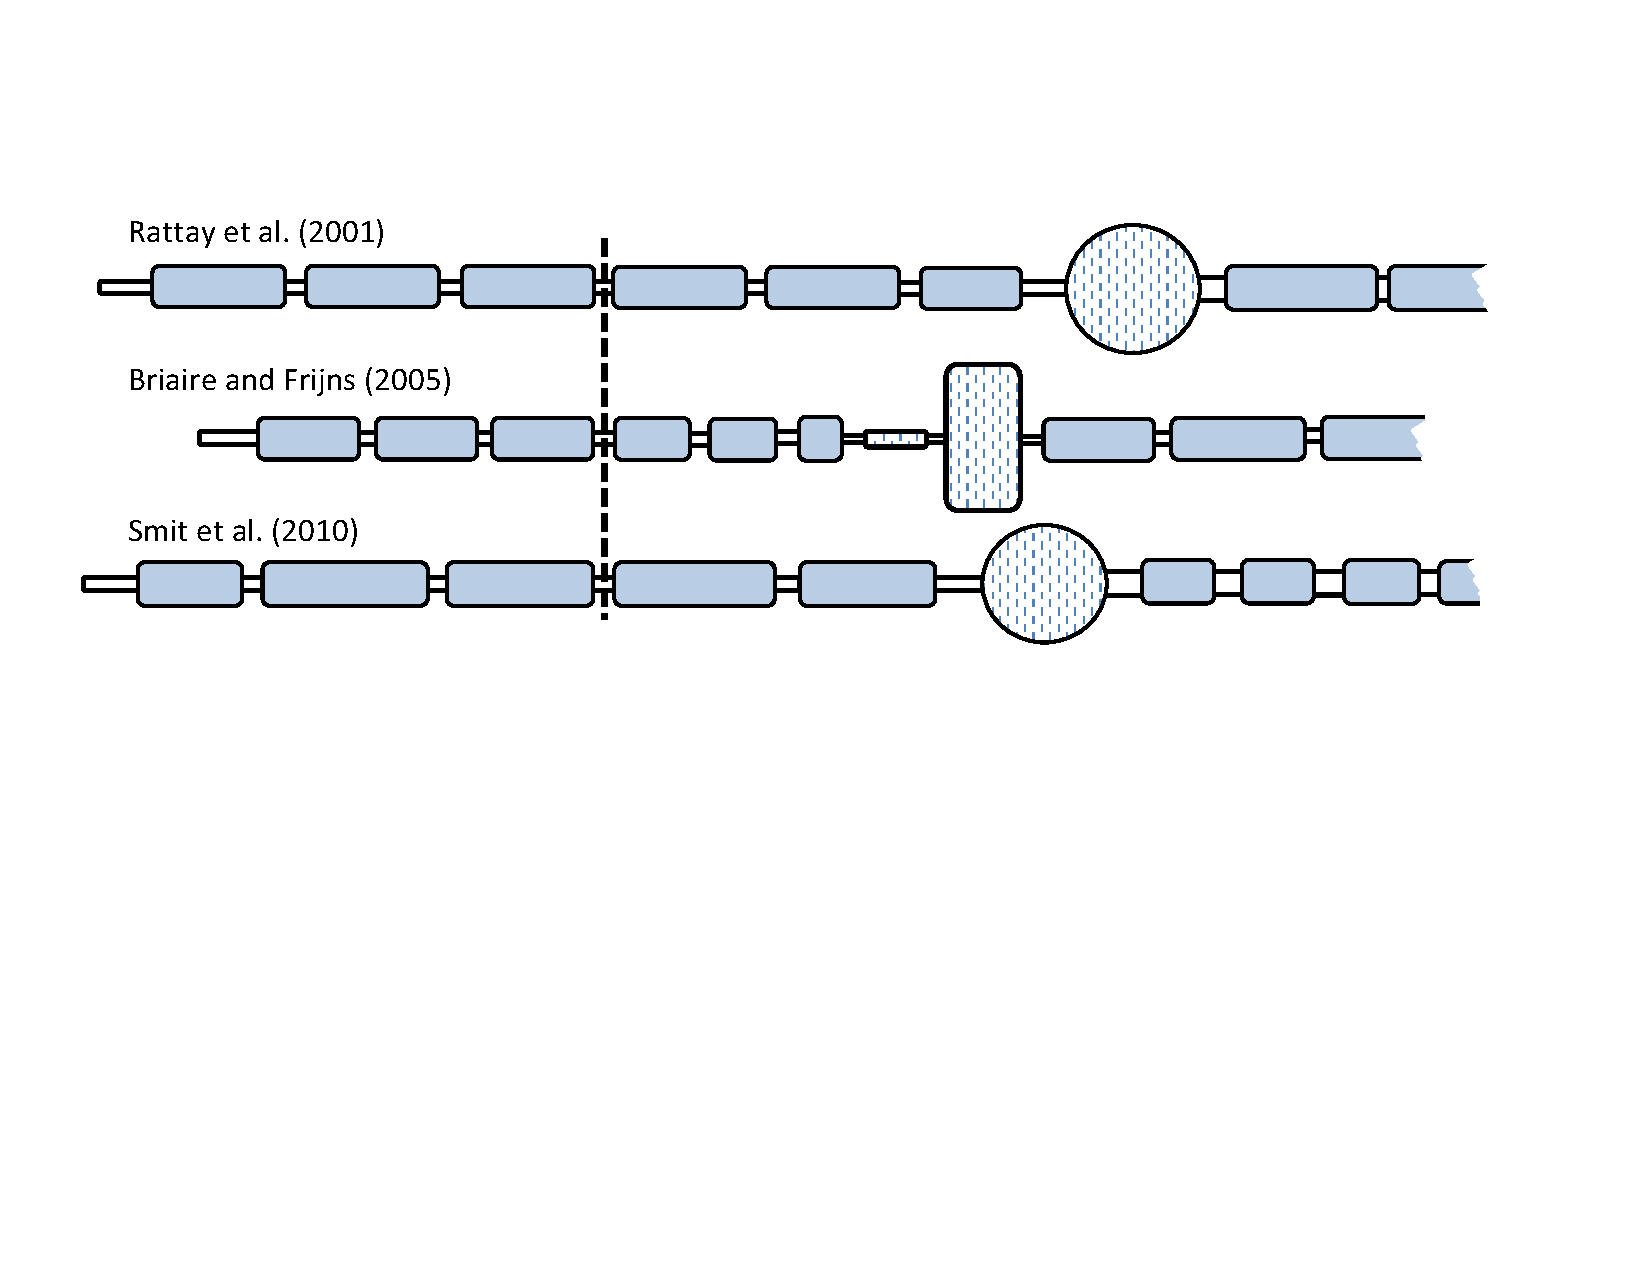
\includegraphics[width=\linewidth]{images/Morphologies.pdf}
\end{center}
\caption{Comparison of the ANF morphologies. All dendrites and axons were myelinated, denoted by the blue color. The somas of all three models were unmyelinated but surrounded by layers of ``satellite cells", as described in \cite{Rattay2001}, and so was the pre-somatic region of the BF model.
Relative differences in compartment size among the three models are indicated in the figure, but they are not true to scale. Vertical line indicates the position of the stimulation electrode (distance from the neuron was \SI{500}{\micro\meter}).
}
\label{fig:morphologies}
\end{figure}

\begin{figure}[h!]
\begin{center}
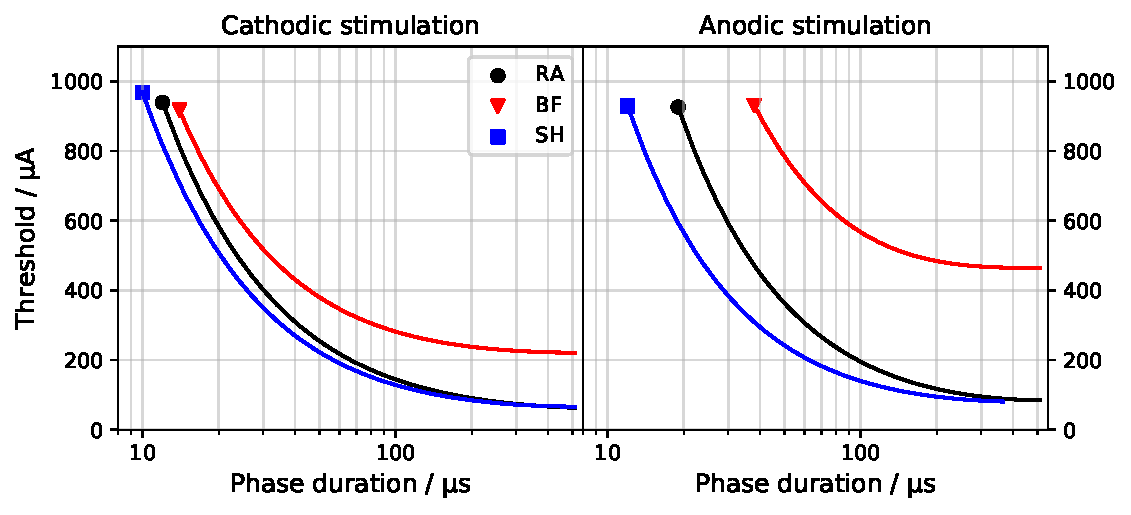
\includegraphics[width=\linewidth]{images/strength_duration_curve_comparison.pdf}
\end{center}
\caption{Strength-duration curves for monophasic cathodic (left) and anodic (right) stimuli. ``RA'', ``BF'' and ``SH'' denote the Rattay, Briaire-Frijns and Smit-Hanekom models, respectively. The $x$-axis is set in a log-scale for a better comparison.}
\label{fig:Strength_duration_curve_comparison}
\end{figure}

\begin{figure}[h!]
\begin{center}
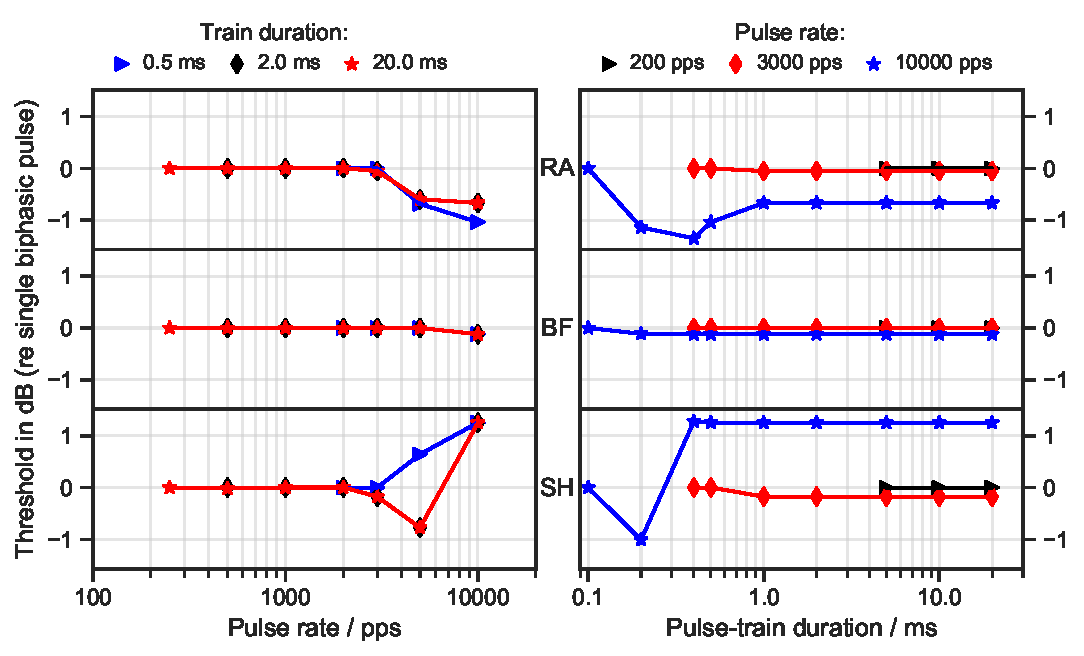
\includegraphics[width=\linewidth]{images/thresholds_for_pulse_trains.pdf}
\end{center}
\caption{Threshold as a function of pulse rate (left column) and pulse-train duration (right column). \textbf{RA}: Rattay model; \textbf{BF}: Briaire-Frijns model; \textbf{SH}: Smit-Hanekom model. The stimulation current was a train of biphasic cathodic-first \SI{45}{\micro\second} pulses with an inter-phase gap of \SI{8}{\micro\second}. The threshold is reported in dB as the ratio of $I_{\T{th}}$ for the pulse train to $I_{\T{th}}$ for a single biphasic pulse.}
\label{fig:thresholds_for_pulse_trains}
\end{figure}
% remove the box around the legends, use different colors or symbols its otherwise confusing that you normally use these colors and symbols to code for the models but here where they code different conditions. Also write to spell Threshold in full

\begin{figure}[h!]
\begin{center}
  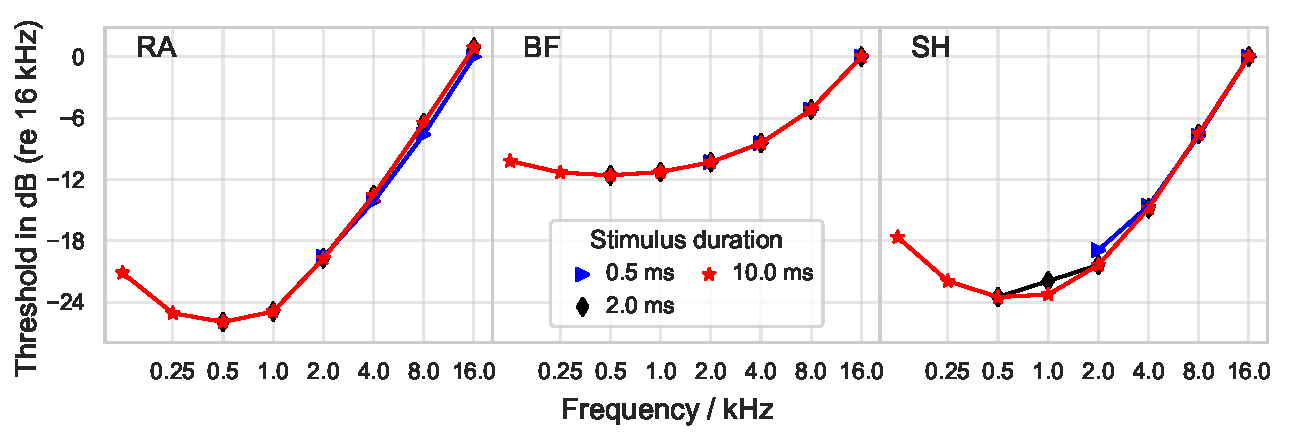
\includegraphics[width=\linewidth]{images/thresholds_for_sinus.pdf}
\end{center}
\caption{Threshold for sinusoidal stimulation as a function of stimulus frequency. The threshold is reported in dB as the ratio to $I_{\T{th}}$ at the frequency of \SI{16}{\kilo\hertz}. ``RA'', ``BF'' and ``SH'' denote the Rattay, Briaire-Frijns and Smit-Hanekom models, respectively. All results are plotted for three stimulus durations.}
\label{fig:thresholds_for_sinus}
\end{figure}
% Same comment on colors and symbols as for the previous graphic

\begin{figure}[h!]
\begin{center}
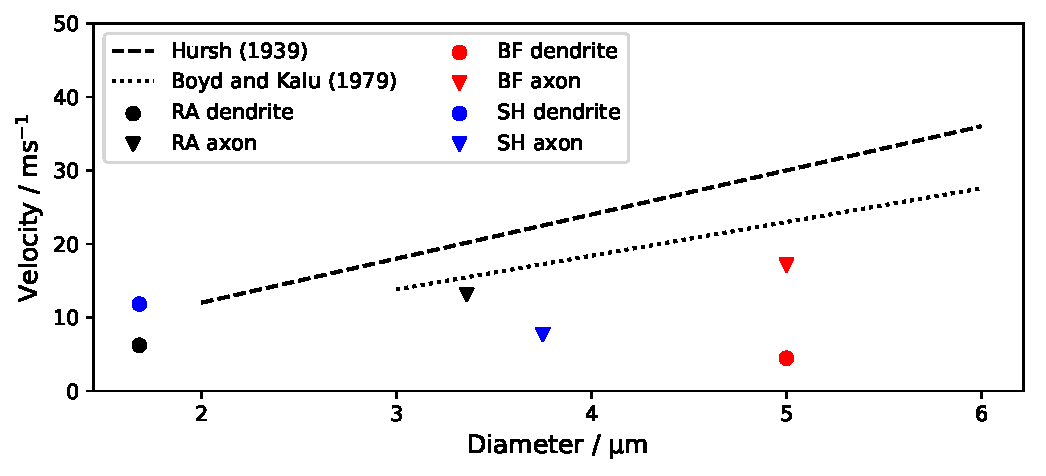
\includegraphics[width=\linewidth]{images/conduction_velocity_plot.pdf}
\end{center}
\caption{Conduction velocity $v_{\T{c}}$ of ANF models in comparison to experimental data. The velocities of dendrite and axon of each model were measured separately due to their morphological and physiological differences. $v_{\T{c}}$ is plotted against the fiber outer diameters. ``RA'', ``BF'' and ``SH'' denote the Rattay, Briaire-Frijns and Smit-Hanekom models, respectively.}
\label{fig:conduction_velocity_plot}
\end{figure}

\begin{figure}[h!]
\begin{center}
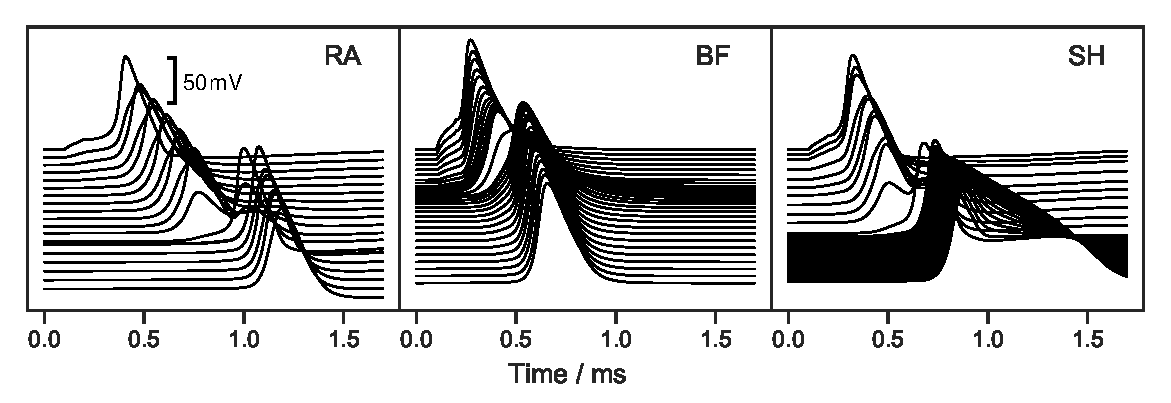
\includegraphics[width=\linewidth]{images/voltage_course_comparison_plot.pdf}
\end{center}
\caption{Response of ANF models to a \SI{100}{\micro\second} cathodic current pulse injected at the peripheral terminal. ``RA'', ``BF'' and ``SH'' denote the Rattay, Briaire-Frijns and Smit-Hanekom models, respectively. Each line depicts the voltage over a course of time at a single morphologic component, starting from the peripheral terminal represented by the topmost line. %Maybe include a very small 100us pulse to represent the current injection
The lines are vertically aligned true to scale according to the compartmental distances.
%The visible delay in the AP propagation is the consequence of a highly capacitive soma.
The high capacitance of the causes a large additional delay of the AP.}
\label{fig:somatic_delay}
\end{figure}

\begin{figure}[h!]
\begin{center}
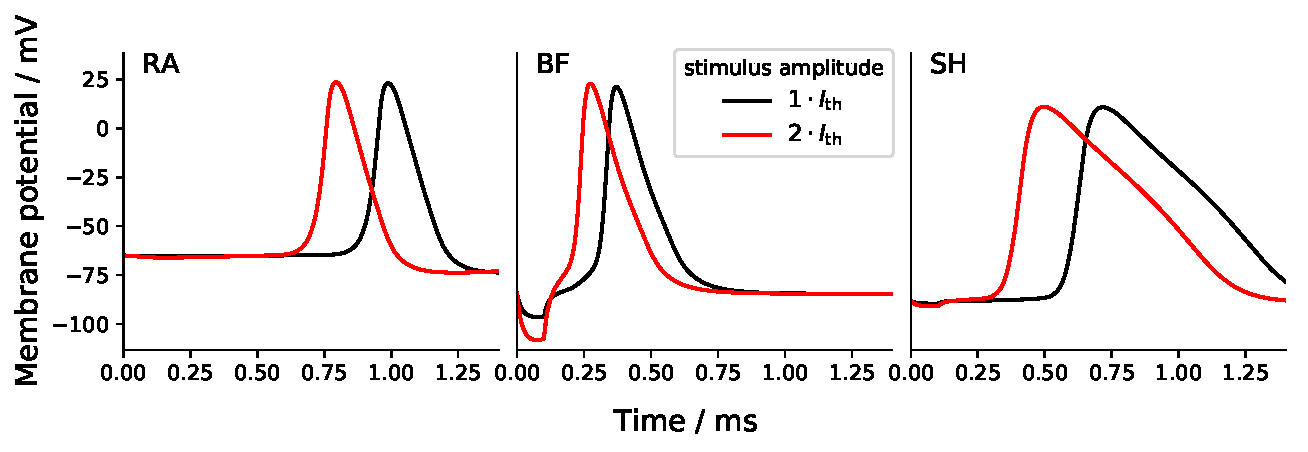
\includegraphics[width=\linewidth]{images/single_node_response_comparison.pdf}
\end{center}
\caption{Transmembrane voltage (action potential) at the tenth axonal node of the ANF models to a monophasic \SI{100}{\micro\second} cathodic current pulse with an amplitude of $I_{\T{rh}}$ and $2\times I_{\T{rh}}$. ``RA'', ``BF'' and ``SH'' denote the Rattay, Briaire-Frijns and Smit-Hanekom models, respectively.}
\label{fig:single_node_response_figure}
\end{figure}
% different colors again. :D just check for consistency

\begin{figure}[h!]
\begin{center}
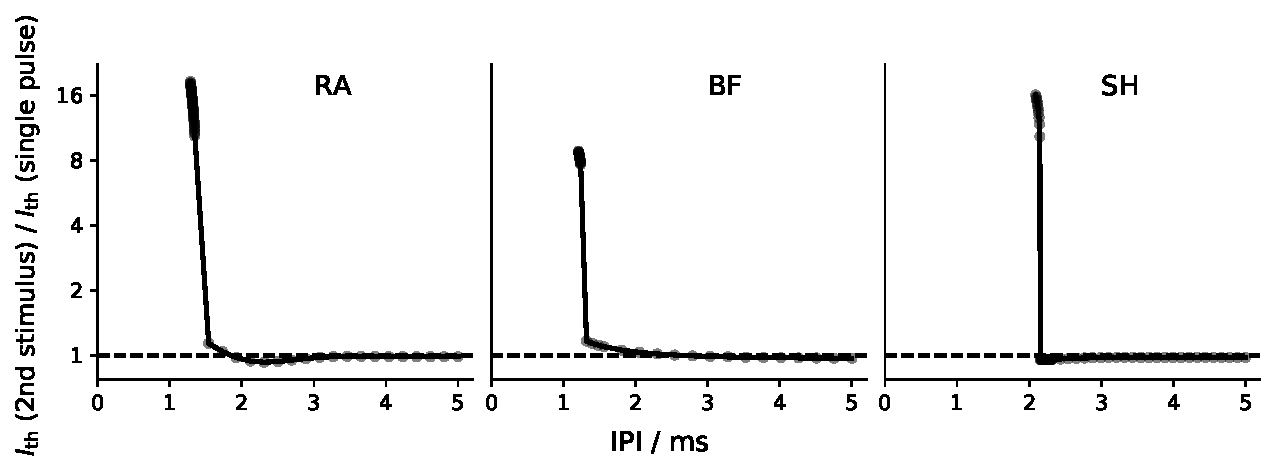
\includegraphics[width=\linewidth]{images/refractory_curves_plot_comparison.pdf}
\end{center}
\caption{Refractory curve of ANF models. Both the masker and the second stimulus were a monophasic cathodic pulse with a phase length of \SI{50}{\micro\second}. ``RA'', ``BF'' and ``SH'' denote the Rattay, Briaire-Frijns and Smit-Hanekom models, respectively. Please notice that the scaling of the $y$-axis is logarithmic.}
\label{fig:refractory_curves}
\end{figure}

\begin{figure}[h!]
\begin{center}
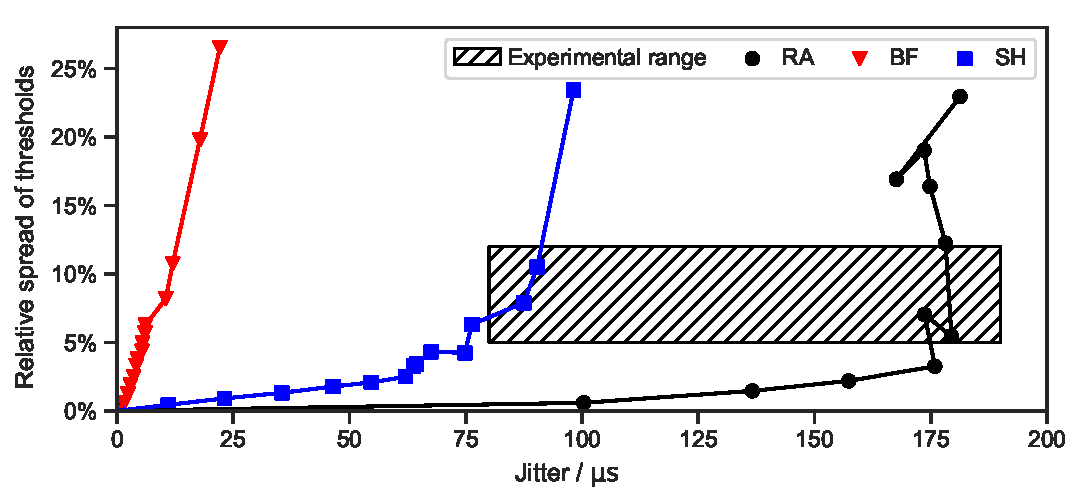
\includegraphics[width=\linewidth]{images/stochasticity_plot.pdf}
\end{center}
\caption{Stochasticity of ANF models with a Gaussian noise current term. Jitter and relative spread of threshold were measured for different values of $k_{\T{noise}}$. A monophasic \SI{50}{\micro\second} cathodic current pulse was applied in each simulation. Threshold and latency were measured 100 and 500 times, respectively,  for each datapoint.
``RA'', ``BF'' and ``SH'' denote the Rattay, Briaire-Frijns and Smit-Hanekom models, respectively. The experimental range was summarised from a series of animal experiments, including \cite{VandenHonert1984}, \cite{Javel1987}, \cite{Dynes1996}, \cite{Miller1999} and \cite{Cartee2000}.}
\label{fig:stochasticity_plot}
\end{figure}

\begin{figure}[h!]
\begin{center}
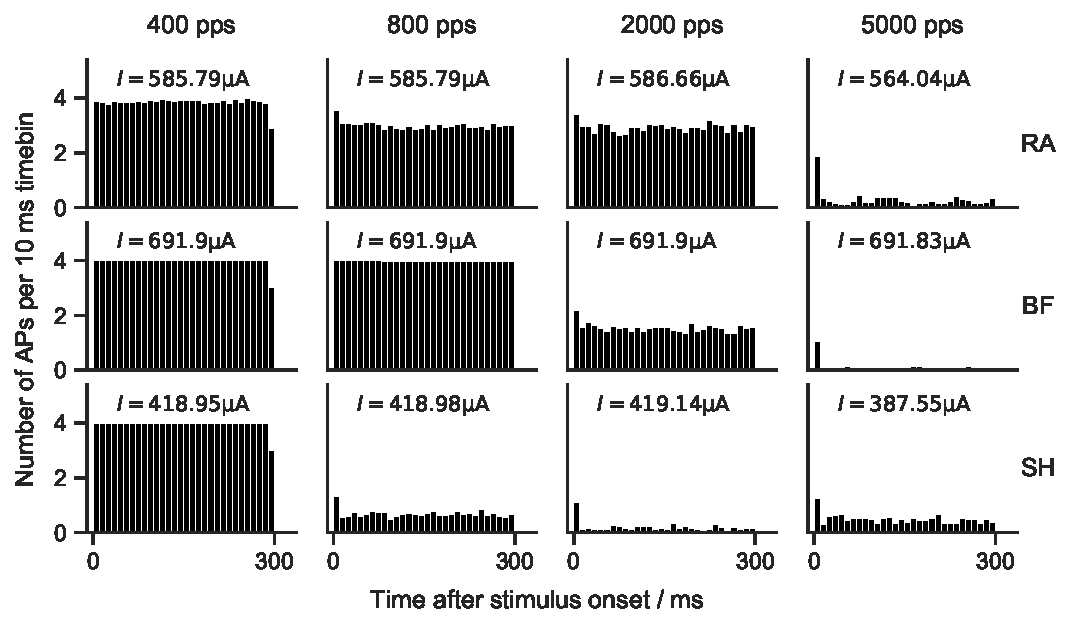
\includegraphics[width=\linewidth]{images/psth_plot_comparison_thr.pdf}
\end{center}
\caption{Poststimulus time histograms of ANF models to \SI{300}{\milli\second} pulse-train stimulation. \textbf{RA}: Rattay model; \textbf{BF}: Briaire-Frijns model; \textbf{SH}: Smit-Hanekom model. Biphasic (cathodic-first) current pulses with a phase duration of \SI{20}{\micro\second} and an amplitude of $I_{\T{th}}$ were used for pulse-trains with four different pulse rates. Each stimulation was repeated 50 times. Vertical columns in PSTHs show the average number of APs in a \SI{10}{\milli\second} time bin.}
\label{fig:PSTH_comparison}
\end{figure}

%%% If you are submitting a figure with subfigures please combine these into one image file with part labels integrated.
%%% If you don't add the figures in the LaTeX files, please upload them when submitting the article.
%%% Frontiers will add the figures at the end of the provisional pdf automatically
%%% The use of LaTeX coding to draw Diagrams/Figures/Structures should be avoided. They should be external callouts including graphics.

\end{document}
